\chapter{Problemanalyse}

TODO: Abschnitt neu schreiben

Die Zusammenführung der Arbeit von mehr als einem Entwickler ist ein komplexer und nicht trivialer Vorgang. \\
Viele Teile eines Softwareprojektes beeinflussen andere und häufig werden an Schnittstellen in Programmen Änderungen von mehreren Entwicklern vorgenommen. \\
Es muss sichergestellt werden, dass die Änderungen zusammengeführt werden können und dass das Ergebnis syntaktisch und semantisch korrekt ist, sowie den Anforderungen entspricht.

Während die syntaktische und semantische Validierung klassische Themen der theoretischen Informatik sind, erfordert die Erhebung und Aufbereitung von Anforderungen eine ganz eigene Betrachtung durch ein konkretes Anforderungsmanagement.

Gerade wenn die Software einen gewissen Umfang übersteigt, ist daher ein solides Anforderungsmanagement essenziell. Zudem müssen Mechanismen geschaffen werden, um sicherzustellen, dass diese Anforderungen über die komplette Laufzeit der Software erfüllt bleiben. 

Leider sieht die Realität in der Softwareentwicklung nicht selten anders aus. Fehlende, nicht dokumentierte oder veraltet Anforderungen sind keine Seltenheit.\\
Ebenso sind lange Zeitintervalle in denen sich Teile der Software in keinem lauffähigen oder einem fehlerbehaftetem Zustand befinden häufig anzutreffen.

Fehlende Anforderungen und fehlerhafte Umsetzungen werden häufig erst zum Zeitpunkt des Testes - oder schlimmer - zum Zeitpunkt der Auslieferung offenbart.

Die Gründe für diese Schwierigkeiten sind häufig in kein homogenes Bild zu bringen. Vielmehr tragen verschiedene Faktoren dazu bei, die erst in der Kombination zu erheblichen Problemen führen können.

\section{Vorgehensmodelle}

Um komplexe Software in einer strukturierten und definierten Herangehensweise zu erstellen, wurden ausführlich
beschriebene und wohl definierte Vorgehensmodelle erarbeitet. Deren Ziel ist es eine klare Schrittfolge mit 
eindeutigen Zielstellungen vorzugeben. Diese Schritte gliedern den komplizierten und komplexen Entwicklungsprozess 
in klar abgegrenzte und bewertbare Abschnitte. 

Die bekanntesten Vorgehensmodelle halten sich an eine klare Folge aus Planungs-,\\ Konzeptions-, Implementierungs-, 
Test- und Abnahmephase. Durch die klare Trennung der Phasen werden diese Modelle auch statische Vorgehensmodelle genannt.
Beispiele sind hier das Wasserfallmodell[quote Wasserfallmodell] und das V-Modell[quote V-Modell]. Insbesondere in
Bereichen mit hohen Sicherheitsanforderungen und einer starken Bindung an bürokratische Strukturen wird auch heute noch
das V-Modell erfolgreich eingesetzt[quote Referenz Bund].

Mit der Komplexität einer Softwareanwendung steigt ihr Umsetzungsaufwand. Dieser zusätzliche Aufwand teilt sich in
statischen Vorgehensmodellen in die einzelnen Phasen auf. Bei besonders umfangreichen Softwareprojekten entsteht daher
eine signifikante zeitliche Diskrepanz zwischen den Phasen der Anforderungsaufnahme und deren Umsetzung. 
Zudem ist der Vorgang der Anforderungsaufnahme ohnehin schwierig ist und kann nur schwer auf Vollständigkeit geprüft
werden. Diese beiden Faktoren erhöhen das Risiko eine fehlerhafte Softwareanwendung zu erstellen. Aus der hohen Dauer der
einzelnen Phasen ergibt sich zudem eine hohe Reaktionszeit um fehlerhaft umgesetzte Anforderungen zu korrigieren.

Ein Projekt zur Umsetzung einer komplexen Softwareanwendung benötigt ein umfangreiches Risikomanagement, um Folgekosten 
zu verringern.

Um den Aufwand für das Risikomanagement und die Folgekosten zu minimieren entwickelte sich eine alternative
Herangehensweise, welche vor allem Interaktion, Funktionalität, Kundenorientierung und Veränderungsbereitschaft als
wichtig erachtet. Festgehalten im Agilen Manifest\footcite{agile-manifest} proklamierten viele bekannte und angesehene
Softwareexperten ihren Willen, Softwareprojekte grundsätzlich anders zu fokussieren.

Beeinflusst von der Lean-Bewegung aus der Automobil-Fertigungsindustrie\footcite{kent1999} wurden die abgegrenzten Phasen 
in den statischen Vorgehensmodellen in Frage gestellt. Hohe Eigenverantwortung und kurze Kommunikationszyklen sind die 
Basis des neuen Vorgehens.

Die Prinzipien des ``Agilen Manifestes'' stellen hohe Ansprüche an Entwickler und erzwingen ein Umdenken im Umgang mit dem Projektprozess. Während in den statischen Vorgehensmodellen jede Phase eine längere zeitliche Periode einnimmt, so werden diese Phasen in agilen Vorgehen deutlich verkürzt und verschwimmen teilweise. Dadurch werden Kommunikationszyklen verkürzt und Informationsflüsse deutlich beschleunigt.
Durch die schnellere Zyklen sinkt die benötigte Zeit zur Reaktion auf Probleme und Hindernisse. Damit ist es möglich kontinuierlich und zeitnah Verbesserungen für den Entwicklungsprozess und die Softwareanwendung einzubringen. 

Agile Vorgehensmodelle und Techniken aus der Lean-Bewegungen setzen stark auf eine Arbeitseinteilung anhand von Produktmerkmalen(Features)[quote Scrum, quote Kanban]. Der von der agilen Bewegung angestrebte starke Produktfokus und die kurzen Iterationen vereinfachen die Bewertung des Projektprozesses und der verwendeten Hilfsmittel.

Der hohe Fokus auf Produktmerkmale und das Prinzip zur frühen und kontinuierlichen Auslieferung von wertvoller Software\footcite{agile-manifest-principles} helfen die Akzeptanz für die Software zu steigern. Außerdem können falsch interpretierte Anforderungen früher erkannt werden. 

Um die Umsetzung der Anforderungen zu prüfen benötigt es eine Qualitätssicherung. Für komplexe Softwareanforderungen ist die Prüfung der Anforderungen mit sehr hohem Aufwand verbunden, wenn sie manuell ausgeführt wird. Um Anforderungen automatisiert zu prüfen, müssen diese abstrakt formuliert werden. Der damit verbundene Aufwand steigt, wenn sich die Anforderungen häufig ändern. Dies sollte in einer Strategie für die Qualitätssicherung beachtet werden. 

\section{Qualitätssicherung und Softwaretest}

Die Erfüllung der Anforderungen an eine Softwareanwendung sollte durch eine Strategie der Qualitätssicherung sichergestellt sein. Da jede Änderung an der Software die Erfüllung der Anforderungen beeinträchtigen könnte, sollten die Anforderungen nach Änderungen erneut geprüft werden. Da manuelle Prüfungen aufwändig und zeitintensiv sind, sollten sie sich auf wenige Anwendungsszenarien beschränken. Diese Anwendungsszenarien sollten nur schwer oder unzuverlässig durch programmierte Prüfungen abgedeckt werden können.

Programmierte Prüfungen, auch Tests genannt, zu erstellen kann sehr komplex und kompliziert sein. Je nach Softwareanwendung und damit verbundenen Anforderungen, müssen Kompromisse zur Laufzeit, Aussagekraft und Wartbarkeit eines Tests eingegangen werden.
Den jeweiligen Schwerpunkten eines Tests geschuldet, werden Tests auf verschiedenen Abstraktionsebenen der Software ausgeführt. Es wird zunächst zwischen funktionalen und nicht-funktionalen Testkriterien unterteilt.
Bei den funktionalen Test wird weiter zwischen Akzeptanz-, Integrations- und Unittests unterschieden\footcite[S.159][]{software-quality2008}. 

\paragraph{Akzeptanztest}
oder auch Abnahmetests stellen in erster Linie die Erfüllung der definierten Anforderungen sicher. Akzeptanztests werden häufig in der Form von Anwendungsszenarien (Use-Cases) beschrieben. Anwendungsszenarien beschreiben das Zusammenspiel von Systemen, deren Akteuren und Aktionen die zwischen diesen ausgeführt werden. Die Verwendung von technischen Details der Software, wie Datenbankspezifikationen oder konkreten Systemimplementierungen, sollten vermieden werden. Nicht nur erhöht es den Wartungsaufwand dieser Tests, es verschiebt auch den Fokus des Tests, weg von den eigentlich zu prüfenden Anforderungen.

\paragraph{Integrationstests}

dienen der Überprüfung von Schnittstellen. Dabei wird das Verhalten der Schnittstelle auf definierte Ein- und Ausgaben geprüft. Der Fokus der Tests liegt darauf unerwartetes Verhalten beim Zusammenspiel mehrere Komponenten auszuschließen.

\paragraph{Unit-Tests}

werden für Objektklassen- und Methodentests verwendet. Das erwartet Verhalten der zu überprüfenden Einheit(Unit) wird mit dem Unit-Test sichergestellt. Zugleich übernimmt er auch eine dokumentarische Funktion. Durch die Initialisierung der Einheit und der Aufruf ihrer Schnittstelle, wird die Intention ihres Autors deutlich.

Die nicht-funktionalen Testkriterien betreffen Merkmale welche nicht einem einzelnen Anwendungsfall zugeordnet werden können. Es werden Leistungsaspekten und unterbewussten Kriterien geprüft. Solche Merkmale sind zum Beispiel Reaktionszeit der Anwendung, wie viele Aktionen pro Zeiteinheit die Anwendung bewältigen kann und wie gut die Anwendung nutzbar ist (Usability). Nicht-funktionale Tests sollten zudem weiter nach der Möglichkeit der Bewertung ihrer Ergebnisse unterteilt werden. Gut zu bewerten sind Leistungs- und Sicherheitstests. Weniger gut zu bewerten sind Explorativ- und Usability-Tests.

\paragraph{Leistungstests} oder auch Performance-Tests werden genutzt um die Leistungsfähigkeit einer Anwendung zu erproben. Kriterien wie Anfragen pro Zeiteinheit, maximale Anzahl paralleler Anfragen und Reaktionszeit, sowie Anfragedauer werden getestet.
\paragraph{Sicherheitstests} werden genutzt um Schwachstellen einer Anwendung zu finden. Es werden Listen von bekannten Sicherheitsproblemen\footcite{owasp-vulnerability} genutzt und in der Anwendung geprüft.
\paragraph{Explorativ-Tests} werden manuell durchgeführt und versuchen Fehler zu finden, die auf anderen Wegen nicht oder kaum zu entdecken sind.
\paragraph{Usability-Tests} werden ebenfalls manuell durchgeführt und sind aufgrund ihrer subjektiven Natur schwer zu bewerten. Es ist daher üblich auf eine Untergruppe dieser Tests zu prüfen, wie zum Beispiel die Barrierefreiheit einer Anwendung.

Die Abbildung~\ref{agile-testing-quadrants} fasst die verschiedenen Tests anhand der Art der Durchführung und anhand ihrer Stackeholder-Ausrichtung in vier Quadranten zusammen\footcite[The Agile testing matrix][]{cd-docker-jenkins}.

\begin{figure}[htbp]
  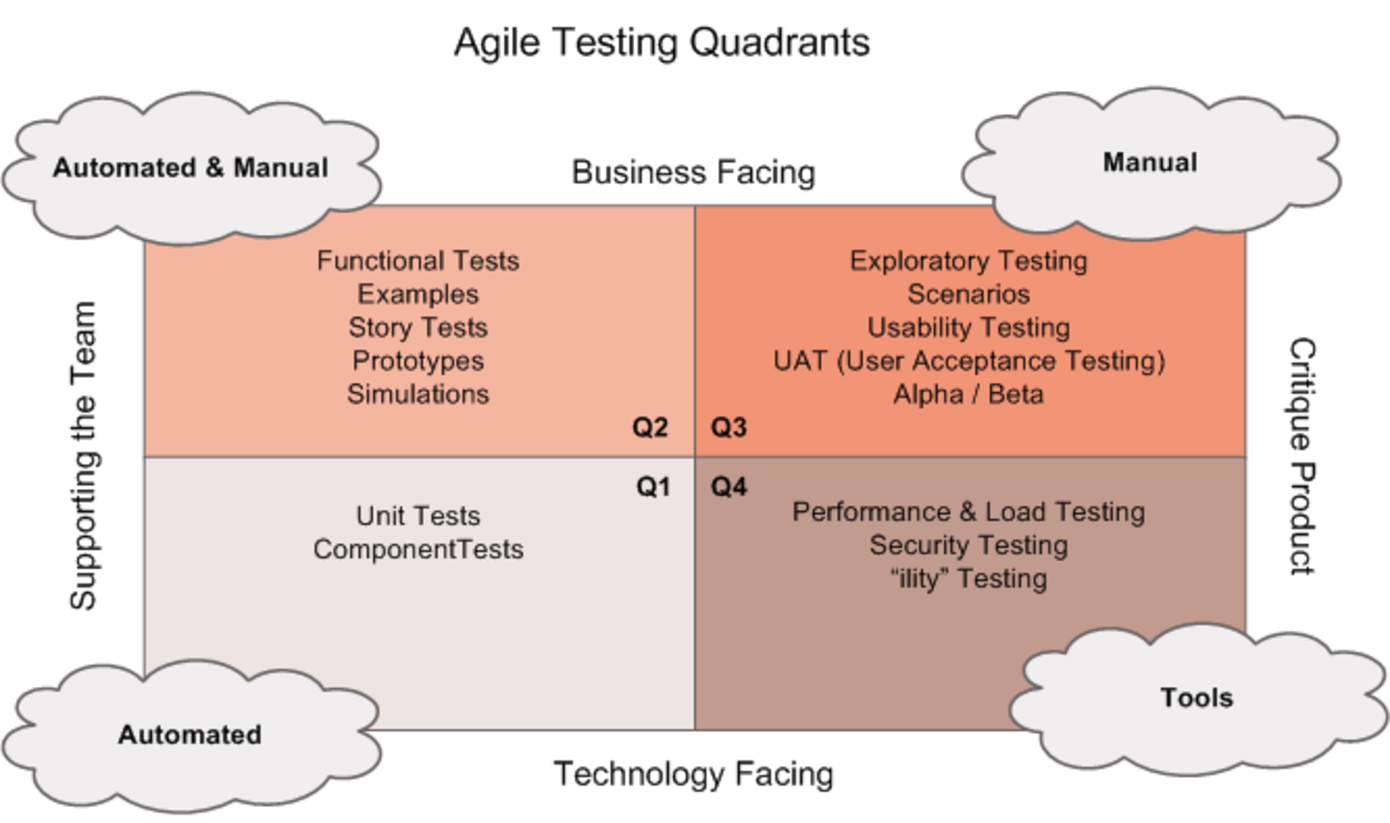
\includegraphics[
    width=\textwidth,
    height=\textheight,
    keepaspectratio
  ]{resources/Agile-Testing-Quadrants.pdf}
  \caption{Agile Testing Quadrants}
  \label{agile-testing-quadrants}
\end{figure}

\section{Automatisierung der Softwareerstellung}
\label{sec:automation-software}

Zur Bereitstellung einer Softwareanwendung werden mehrere Schritte benötigt. Es wird ein konkreter Stand der Softwarequellen benötigt, ein ausführendes System und es muss für eine Kompilierung der Softwarequellen zu dem System gesorgt werden.
Je nach Anforderung und Art der Softwareanwendung entspricht dieser Vorgang einer trivialen Kopie oder einem mehrstufigen, komplexen Vorgang. 

Im Nachfolgenden wird beschrieben wie Software in einen wohldefinierten, funktionalen Zustand gebracht und dieser validiert wird. Dazu wird auf Versionsverwaltungssysteme, Konfigurationsmanagement, die automatisierte Erstellung der Softwareanwendung und deren Test eingegangen.

\subsection{Codeverwaltung und Versionsverwaltungssysteme}

Programmversionen können bei fast jeder käuflich zu erwerbenden Softwareanwendung unterschieden werden. Potentielle 
Anwender konnten so bereits vor Erwerb transparent nachvollziehen, wie fortschrittlich die Anwendung war.
Für die Entwicklung ergab sich daraus die Herausforderung Fehlerkorrekturen nach Veröffentlichung der Software, für viele 
verschiedene Programmversionen bereit zustellen.
Eine nachvollziehbare und leicht zu verwendende Ablage der einzelnen Programmversionen war daher sehr hilfreich.

Die einfachste Form der Ablage ist eine manuelle Kopie der Softwareanwendung. Mit der Weiterentwicklung der Anwendung und 
dem Entstehen weiterer Programmversionen zeigen sich schnell schwächen dieses Systems. Wenn in einer frühen 
Programmversion ein Fehler gefunden und behoben wird, sollte dieser auch in allen anderen folgenden Versionen behoben 
werden. Dadurch entsteht mit dieser einfachen Ablage ein erheblicher Mehraufwand. Fortschrittliche 
Versionsverwaltungssysteme bieten Möglichkeiten diesen Mehraufwand zu reduzieren.

Zustandssicherheit ist ein besonders wichtiges Merkmal für Versionverwaltungs- oder auch Versionskontrollsysteme.
Die Reproduzierbarkeit eines definierten Zustandes der Softwarequellen. Der definierte Zustand der Anwendung ergibt sich 
aus der Abfolge aller Änderungen, die an der Softwareanwendung vorgenommen wurden, bis zu der jeweiligen Programmversion. 

Als weiteres Merkmal ist die Transparenz aller getätigten Änderungen anzuführen. Die Nachvollziehbarkeit der Änderungen 
ist hilft oft bei der Koordinierung der Entwicklung mit mehreren Programmieren. Außerdem ist es sehr hilfreich zu wissen, 
welcher andere Projektteilnehmer bei Problemen mit einem Code-Abschnitt gefragt werden kann. 

Über die Entstehung von Versionsverwaltungssysteme[quote Soft.Quali] haben sich vor allem zwei Prinzipien herausgebildet: 
zentrale und dezentrale Versionsverwaltungssysteme. Zwar unterscheiden sich die Versionsverwaltungssysteme auch in 
anderen Merkmalen, zum Beispiel in der Ablage der Quellen und deren Änderungen, diese Merkmale haben aber nahezu keinen 
Einfluss auf die Verwendung im Softwareentwicklungsprozess.

\paragraph{Zentrale Versionsverwaltungssysteme} folgen dem ``single point of truth'' Prinzip. Es existiert nur ein 
zentraler Punkt auf dem alle Versionstände gespeichert werden. Dies ermöglicht einen einfachen Kontrollfluss und führt nur zu geringfügigen Abweichungen unter allen beteiligten Entwicklern. Damit einhergehend ist eine Übersicht aller Änderungen problemlos möglich.

Nachteil dieser Variante ist häufig der initiale Aufwand, da eine zentrale Komponente bereitgestellt werden muss. Zudem 
sind zentrale Systeme generell störanfälliger und weniger Ausfallsicher. Der Vorteil des ``single point of truth'' führt 
auch zum Nachteil des ``single point of failure'', wodurch Probleme alle Teilnehmer gleichzeitig betreffen.
Je nach verwendeter Versionierungsstrategie kann es zudem zu einer zentralen Sperrung einzelner Bereiche der Softwarequellen kommen, wenn diese für eine exklusive Bearbeitung gesperrt werden.

\paragraph{Dezentrale Versionsverwaltungssysteme} benötigen im Gegensatz keine zentrale Instanz und können problemlos in 
einem losen Verbund von Einzelsystemen betrieben werden. 
Durch die optionale Verwendung einer zentralen Instanz, ergibt sich eine hohe Flexibilität für den Entwickler. Änderungen 
können vom Entwickler nach belieben verschoben und kombiniert werden.
Häufig werden jedoch Restriktionen hingenommen, die ein kontrolliertes gemeinsamen Arbeiten ermöglichen. Beim gemeinsame 
Arbeiten ist besonders auf die Veränderung bereits geteilter Inhalte zu achten.
 
Dezentrale Systeme verwalten jeweils eigenständig eine Kopie der geteilten Inhalte. Dadurch ergibt sich eine hohe 
Redundanz, welche sich positiv auf die Ausfallsicherheit und Verfügbarkeit der Inhalte auswirkt. Im Gegensatz dazu 
entsteht ein Mehraufwand bei der Koordinierung der Einzelsysteme.

\subsection{Konfigurationsverwaltung}
\label{subsec:konfigurationsverwaltung}

Konfigurationsverwaltung ist eine wichtige Basis für die automatisierte Erstellung eines Softwareprojektes. Sie definiert 
wie alle Teilstücke, auch Artefakte genannt, in einem Softwareprojekt miteinander interagieren. Im Detail wird dabei 
Erstellung, Identifikation, Validierung und Ablage geregelt. Die Definition und Konfiguration der Ausführungsumgebung der 
Artefakte ist ebenso ein Teil des Konfigurationsmanagement. \footcite{humble2010}

Ein lockerer Umgang mit der Konfigurationsverwaltung kann gerade zu Beginn eines Projektes ohne nennenswerte Folgen 
einhergehen. Spätestens aber während der Weiterentwicklung der Softwareanwendung sind Folgen deutlich zu spüren. Hierbei 
wird auch von der Alterung des Softwaresystem gesprochen.\footcite{software-quality2008}. Gerade wenn sich unbemerkt die 
Version oder Konfiguration der Software eines Drittanbieters ändert, kann dies schwer zu identifizierende Probleme nach 
sich ziehen. In anderen Fällen reicht es allerdings auch, wenn sich die Konfiguration zwischen Entwicklungs- und 
Produktivumgebung leicht unterscheidet. Konfigurations- und Abhängigkeitsfehler können leicht einen sehr hohen 
Behebungsaufwand verursachen.

Im Idealfall kann eine vollständige Konfigurationsverwaltung:
\begin{itemize}
\item ein durch Betriebssystem und installierte Anwendungen definiertes System bereitstellen, wobei Versionen und Konfiguration alle Elemente Teil der Definition sind.
\item auf jeder Umgebung jeden dieser Bestandteile einzeln inkrementell verändern und diese Änderungen über alle Systeme synchronisieren.
\item alle Änderungen mit Zeitpunkt und Verursacher einfach darstellen
\item Sicherheitsregeln und Konventionen über alle Systeme sicherstellen
\item alle diese Funktionalitäten barrierefrei dem Entwicklungsteam zur Verfügung stellen
\end{itemize}

Alle Forderungen sind nicht immer notwendig, helfen allerdings erheblich bei der Wartung und Betreuung der einzelnen Systeme. 
Eine Virtualisierung der Systeme und eine Versionsverwaltung der zugehörigen Konfiguration und Scripte ist ebenfalls 
hilfreich. Ein solches System kann gut Skalieren und ist mit geringen Aufwand zu handhaben.\footcite{humble2010}

\subsection{Abhängigkeitsverwaltung}

In der Abhängigkeitsverwaltung werden die Softwareabhängigkeiten der Anwendung beschrieben. In auf  Komponenten 
basierenden Anwendungen schließt dies die eigenen, internen Abhängigkeiten mit ein. Diese Abhängigkeiten, meist Module 
genannt, sollen die mit monolithischen Strukturen einhergehenden Nachteile unterbinden. Monolithen weisen häufig eine 
schwache Softwarearchitektur auf und entwickeln sich daher entsprechend schlecht weiter. Mögliche Skalierungen des 
Systems oder ein Austausch von einzelnen Bestandteilen sind mit einem erheblichen Mehraufwand verbunden.

Die Aufteilung einer Anwendung auf mehrere Komponenten erhöht hingegen die Skalierbarkeit und Austauschbarkeit. Zudem 
ergeben sich Vorteile für das verteilte Arbeiten von Teams. 
Eine zu starke Aufteilung der Anwendungsstruktur oder eine Teilung an der falsche Stelle, kann hingegen zu gegenteiligen 
Effekten führen. Ein deutlicher Mehraufwand und eine schlechte Skalierbarkeit sind die Folge. Um die verschiedenen Module 
und Pakete zu organisieren empfiehlt sich eine Abhängigkeitsverwaltung. Diese lassen Abhängigkeitsbeschreibungen anhand 
von Versionsnummern. Dadurch lassen sich Schwierigkeiten unter den Abhängigkeiten leichter erkennen und Versionsupdates 
entsprechend der Abhängigkeiten vornehmen.

Für die automatisierte Erstellung der Softwareanwendung ist es erforderlich, ähnlich wie bereits bei der 
Versionsverwaltung, ein eindeutiges Abhängigkeitsnetz zu beschreiben. Zum Auflösen der Abhängigkeiten werden meist 
mehrdeutige Ausdrücke verwendet werden, die eine Bandbreite an Versionen der Abhängigkeiten erlauben. Wird die Anwendung 
erstellt und Ausgeliefert, sollte allerdings eindeutig sein, welche Abhängigkeiten verwendet werden. Daher werden in 
vielen Packetverwaltungen diese Informationen in einre Lock-Datei festgehalten. Es wird zudem angeraten diese Datei in 
die Versionkontrolle aufzunehmen.\footcite{composer-why-lock-in-vcs}

\subsection{Automatisierte Erstellung und Auslieferung}

Viele Softwareanwendungen müssen kompiliert werden um von einem System ausgeführt werden zu können. Die Kompilierung von kleine Programmen ist eine schnelle und wenig aufwändige Aufgabe. Durch das Wachstum einer Softwareanwendung und das hinzukommen weiterer Abhängigkeiten und Konfiguration wird die Ausführung deutlich zeitintensiver und es werden mehr Einzelschritte benötigt. Der vollständige Ablauf wird dann im Allgemeine Build genannt. Die beim Build ausgeführten Ablaufbeschreibungen Build-Skripte. 

Build-Scripte die mit der Anwendung zusammen wachsen und an Komplexität gewinnen, stellen ein Risiko dar. Die Skripte sollten als Teil der Anwendung verstanden werden und gleichwertigen Qualitätskriterien unterzogen werden. Nur wenig gewartet Build-Skripte weisen meist eine hohe Komplexität auf. Im Fortgeschrittenen Fall kann dies zur  ``integration angst'' führen. Eine geringe Commit-Frequenz und eine sehr defensive Programmierung sind die Folge und behindern das Voranschreiten der Softwareanwendung deutlich\footcite{ci-is-not-build-systems}.

Werden bei einem Erstellungsskript Aspekte der vorangegangen Abschnitte zu Versions-, Konfigurations- und Abhängigkeitsverwaltung nicht berücksichtigt, können zudem inkonsistente und damit nicht 
wiederholbare Resultate erzeugt werden. Diese können zu schwer oder nicht auffindbaren Fehlern führen.

Ziel bei der Erstellung eines Build-Skriptes ist es einen konsistenten und transparenten Ablauf zu 
befolgen. Dies wird unter anderem durch die korrekte Versionsverwaltung der einzelnen Komponenten, Konfigurationen und 
Abhängigkeiten erreicht. Mit diesen Informationen können erstellte Produkte, auch ``build artifacts'' oder Artefakte 
genannt, in einem zentralen Artefakt-Lager abgelegt werden. Dies gewährleistet sowohl einen schnellen Zugriff auf 
Teilartefakte, als auch einen konsistentes Ergebnis bei der Erstellung der Auslieferung.

Die Auslieferung der Software ist direkt mit der Erstellung verwoben. Die Verfügbarkeit aller Abhängigkeiten auf dem 
Zielsystem und die richtige Konfiguration aller Anwendungsbestandteil ist notwendig für die Lauffähigeit der Software. 
Ein vollständiges Konfigurationsmanagement beschreibt die Systemabhängigkeiten und sorgt folglich für die korrekte 
Auslieferung der richtigen Artefakte.

Sowohl bei der Erstellung, als auch bei der Auslieferung ist insbesondere auf eine vollständige Beschreibung der 
notwendigen Schritte zu achten. Gerade auf Entwicklungssystemen können Abhängigkeiten vorhanden sein, welche zwar für die 
Funktionalität der Anwendung sorgen, allerdings nicht beschrieben wurden. Bei der Auslieferung auf andere Systeme können 
diese ``Schattenabhängigkeiten'' dann zu unerwartetem Verhalten oder Abstürzen führen. 
Auch an dieser Stelle bietet sich die Virtualisierung der verwendeten Systeme an. Dadurch kann sichergestellt werden, 
dass die Anwendung immer unter den gleichen, richtigen Bedingungen ausgeführt wird. Wird die Virtualisierungsumgebung 
voll automatisch erstellt, ist zudem gesichert, dass alle Abhängigkeiten beschrieben sein müssen.
Abschließend können diese Umgebungen archiviert und zusammen mit der Programmversion abgelegt werden. Dies unterstützt 
die Konsistenz, Transparenz sowie Skalierbarkeit[quote virtualiserung mit docker] des Entwicklungsprozesses für die 
Anwendung.

Bei der Auslieferung der Software können grob zwei Stufen der Automatisierung unterschieden werden. Eine Stufe ist die 
manuell angestoßene Auslieferung, bei der der Zeitpunkt der Auslieferung davon bestimmt wird, wann das automatisierte 
oder automatisiert-moderierte Script ausgeführt wird. Eine Andere ist die vollautomatisierte Auslieferung, hier wird der 
Zeitpunkt lediglich von der Durchlaufzeit einer Änderung durch die Qualitätskontrolle bestimmt.
Des Weiteren werden unterschiedliche Auslieferungsstrategien (``deployment strategies'') unterschieden, es seien an 
dieser Stelle nur exemplarisch das ``blue green deployment'' und das ``canary deployment''\footcite[261-264 Deploying and Releasing Applications][]
{humble2010} genannt. Die Auslieferungsstrategien werden dabei je nach Anforderungen ausgewählt und haben Vorzüge wie 
Ausfallsicherheit, Bewertung der ausgelieferten Änderung oder Skalierbarkeit der Zielsysteme.

Die konkrete Auslieferung hat auf die Bereiche Continuous-Integration und Feature-Branches nur begrenzt Einfluss. Daher 
werden Continuous-Deployment Strategien nicht weiter betrachtet.

\subsection{Validierung und Test}

Die Validierung einer Software ist ein sehr komplexes Unterfangen. Die vollständige Richtigkeit eines Programmes 
zu beweisen, scheitert bereits bei kleinen Anwendungen, da die Programmkomplexität mit ihrem Umfang stark steigt. Zudem 
können nur Teile validiert und getestet werden, welche im Vorfeld bestimmt worden sind. Unklare, mehrdeutige oder 
fehlende Anforderung machen einen Test unvollständig oder nehmen dem Test die Aussagekraft\footcite[S. 243 Kapitel 4.6][]{software-quality2008}.
\\\\
TODO: einfügen komplexitätstheorie gedumsel
\\\\
Da eine Software nicht in verhältnismäßiger Zeit getestet werden kann, muss eine Strategie gewählt werden. Es muss 
bestimmt werden welche Teile der Anwendung getestet werden. Die Vollständigkeit der Tests, auch Testabdeckung genannt, wird gemessen durch die Nachverfolgung, welche Teile der Softwareanwendung beim Test durchlaufen werden. Bei der Entscheidung welche Strategie gewählt wird, fallen verschiedene Kriterien ins Gewicht. Zum einen muss betrachtet werden, welche Anforderungen mit welchem Testverfahren getestet werden können. Zum anderen welche Granularität für jeden Test verwendet wird.
Je nachdem welche Strategie gewählt wird, hat dies Auswirkungen auf die Ausführungszeit der Tests. Diese Zeit wirkt sich 
direkt auf die Produktivität des Entwicklungsteams aus. Ohne die Testresultate kann kaum eine Aussage über die 
Funktionsfähigkeit der Anwendung getroffen werden. Damit ist die Freigabe einer Softwareanwendung oder eines Inkrementes 
der Anwendung direkt von der Durchlaufgeschwindigkeit der Tests abhängig.

Ein wichtiger Punkt ist hier auch die aktive Wartung der Testsammlung(Test-Suite). Jeder Fehler, der nicht von der Testsammlung erfasst wurde, muss spätestens nach der Beseitigung des Fehlers auch durch die Testsammlung validiert werden. Diese Regressions-Sicherheit stellt in vielen Testsammlungen häufig den größten Teil der Tests\footcite{software-quality2008}. Ein direkter Nachteil einer großen Test-Suite ist der Aufwand für ihre Pflege. Testabdeckung, Wartbarkeit der Tests und Aussagekraft der Tests sollte daher in der Teststrategie gegeneinander abgewogen werden.

\subsubsection{Software-Metriken}
\label{subsubsec:base-metrics}
Software-Metriken können systematisch und quantitativ Aspekte des Software-Codes erfassen. Als Teilaspekt der Code-Analyse können Software-Metriken dazu verwendet werden Kenngrößen des Software-Systems zu quantifizieren und damit Bewertung und Vergleich mit anderen Code-Ständen ermöglichen\footcite[S.247][]{software-quality2008}

Eine nützliche Software-Metrik sollte mehrere Gütekriterien erfüllen. Die Metrik sollte objektiv sein, was bei einer maschinelle Erhebung und Verarbeitung weitestgehend gegeben ist. Die Ergebnisse einer Metrik sollten wiederholbar und damit robust sein. Zudem sollten die Ergebnisse vergleichbar sein, um verschieden Software-Stände gegeneinander bewerten zu können. Eine Metrik sollte mit dem untersucht Merkmal korrelieren. Die Korrelation ist dann besonders hoch, wenn  der mit der Metrik erhobene Wert sich stark ändert und das betrachtet Merkmal ebenfalls. Abschließend sollte die Erhebung der Metrik in Relation zu der Güte ihrer Aussage stehen. Metriken mit einem hohen Erhebungsaufwand, aber ohne Relevanz für den Entscheidungsprozess, sind nicht wertvoll.\footcite[S.248 ff][]{software-quality2008}

Da Tests und Software-Metriken die einzigen Möglichkeiten sind um automatisiert Einschätzungen der Software vorzunehmen, werden diese Bereiche erneut im Kapitel~\ref{subsec:main-metrics} aufgegriffen und näher auf deren Anwendung eingegangen.

Im folgenden werden kurz bekanntere Metriken vorgestellt.\footcite[S.249 ff][]{software-quality2008}

\paragraph{LOC und NCSS} sind Kenngrößen für den Umfang des Sofware-Codes. ``Lines of Code'' (LOC) geben die Anzahl von Code-Zeilen an. ``Non Commented Source Statements'' (NCSS) ist die gleiche Kenngröße, allerdings abzüglich der Kommentarzeilen. Beide Metriken haben nur ein sehr schwache Aussage über den Umfang des Software-Codes.

\paragraph{Halstead-Metrik} ist eine Kenngröße für die Programmkomplexität. Die Ermittlung erfolgt durch die Analyse der lexikalischen Struktur vom Software-Code. Dabei wird der Code in Operatoren und Operanden eingeteilt und deren Auftrittscharakteristik analysiert. Kritik an dieser Metrik entsteht durch die offene Definition von Operanden und Operationen. Als Folge sind verschiedene Programmiersprachen nur bedingt Vergleichbar durch diese Metrik. Des Weiteren wird in Frage gestellt, ob alle Kerngrößen der Metrik überhaupt mit der lexikalischen Analyse ermittelt werden können.

\paragraph{McCabe-Metrik} ist eine weitere Kennzahl für die Programmkomplexität. Zentrale Größe der Metrik ist die ``zyklomatische Komplexität'' als Maß der Anzahl von Kanten und Knoten eines Kontrollflussgraphen der Software-Anwendung. Somit korreliert die zyklomatische Komplexität mit den möglichen Anwendungsdurchläufen und -zuständen.

\paragraph{Komponenten-Metriken} sind eine Sammlung von Umfangs- und Komplexitätsmetriken für objektorientierten Software-Code. Eine Aussage über den Umfang von Klassen wird unter anderem durch die Anzahl von Attributen und Methoden getätigt. Die Komplexität wird durch die Tiefe und Häufigkeit von objektorientierten Techniken gemessen. Diese Techniken sind unter anderem Vererbung, Überladung und Überschreien. Daher lässt sich mit letzteren Metriken auch eine Aussage über die Code-Kopplung vornehmen.

\paragraph{Struktur-Metriken}\label{par:structure-metrics} mit der wichtigsten Untergruppe der Kopplungsmetriken beschreiben ebenfalls die Programmkomplexität. Besonders wichtig sind die Kenngrößen Fan-In und Fan-Out. Fan-Out ist die Anzahl an Verwendungen eine Klasse in anderen Klassen. Fan-In die Anzahl der verwendeten Klassen in einer Klasse. 

\subsubsection{Software-Verifikation}
\label{subsubsec:base-verification}
Verfahren der Software-Verifikation sind die Deduktion, Modellprüfung und der abstrakten Interpretation\footcite[S. 333 ff][]{software-quality2008}. 

\paragraph{Deduktion} ist stark aus der klassischen mathematischen Beweisführung entlehnt. Dabei werden Vor- und Nachbedingung durch Umformungen sukzessive ineinander überführt. Dieses Verfahren ist ein großteils manueller Vorgang.

\paragraph{Modellprüfung} überführt ein Programm in eine Kripke-Struktur, ähnlich einem endlichen Automaten und beweist oder widerlegt diese Struktur mithilfe von Traversierungsalgorithmen. Die algorithmische Komplexität dieses Verfahrens sorgt für eine weitestgehend ausschließliche Anwendung für sicherheitskritische Software-Systeme.

\paragraph{Abstrakte Interpretation} ist eine semi-formale Verifikationstechnik. Sie kombiniert statische Programmanalyse und Generalisierung von Datenbereichen, um verschieden dynamische Eigenschaften eines Programmes zu verifizieren.

Für die vollautomatische Betrachtung von Software-Änderungen eignet sich daher nur die abstrakte Interpretation und die bereits beschriebenen Software-Tests. Die Abbildung~\ref{software-quali-verification} stellt noch einmal übersichtlich das Verhältnis von Ausdrucksstärker und Skalierbarkeit der Verifikationstechniken dar\footcite[S. 337][]{software-quality2008}.

\begin{figure}[htbp]
  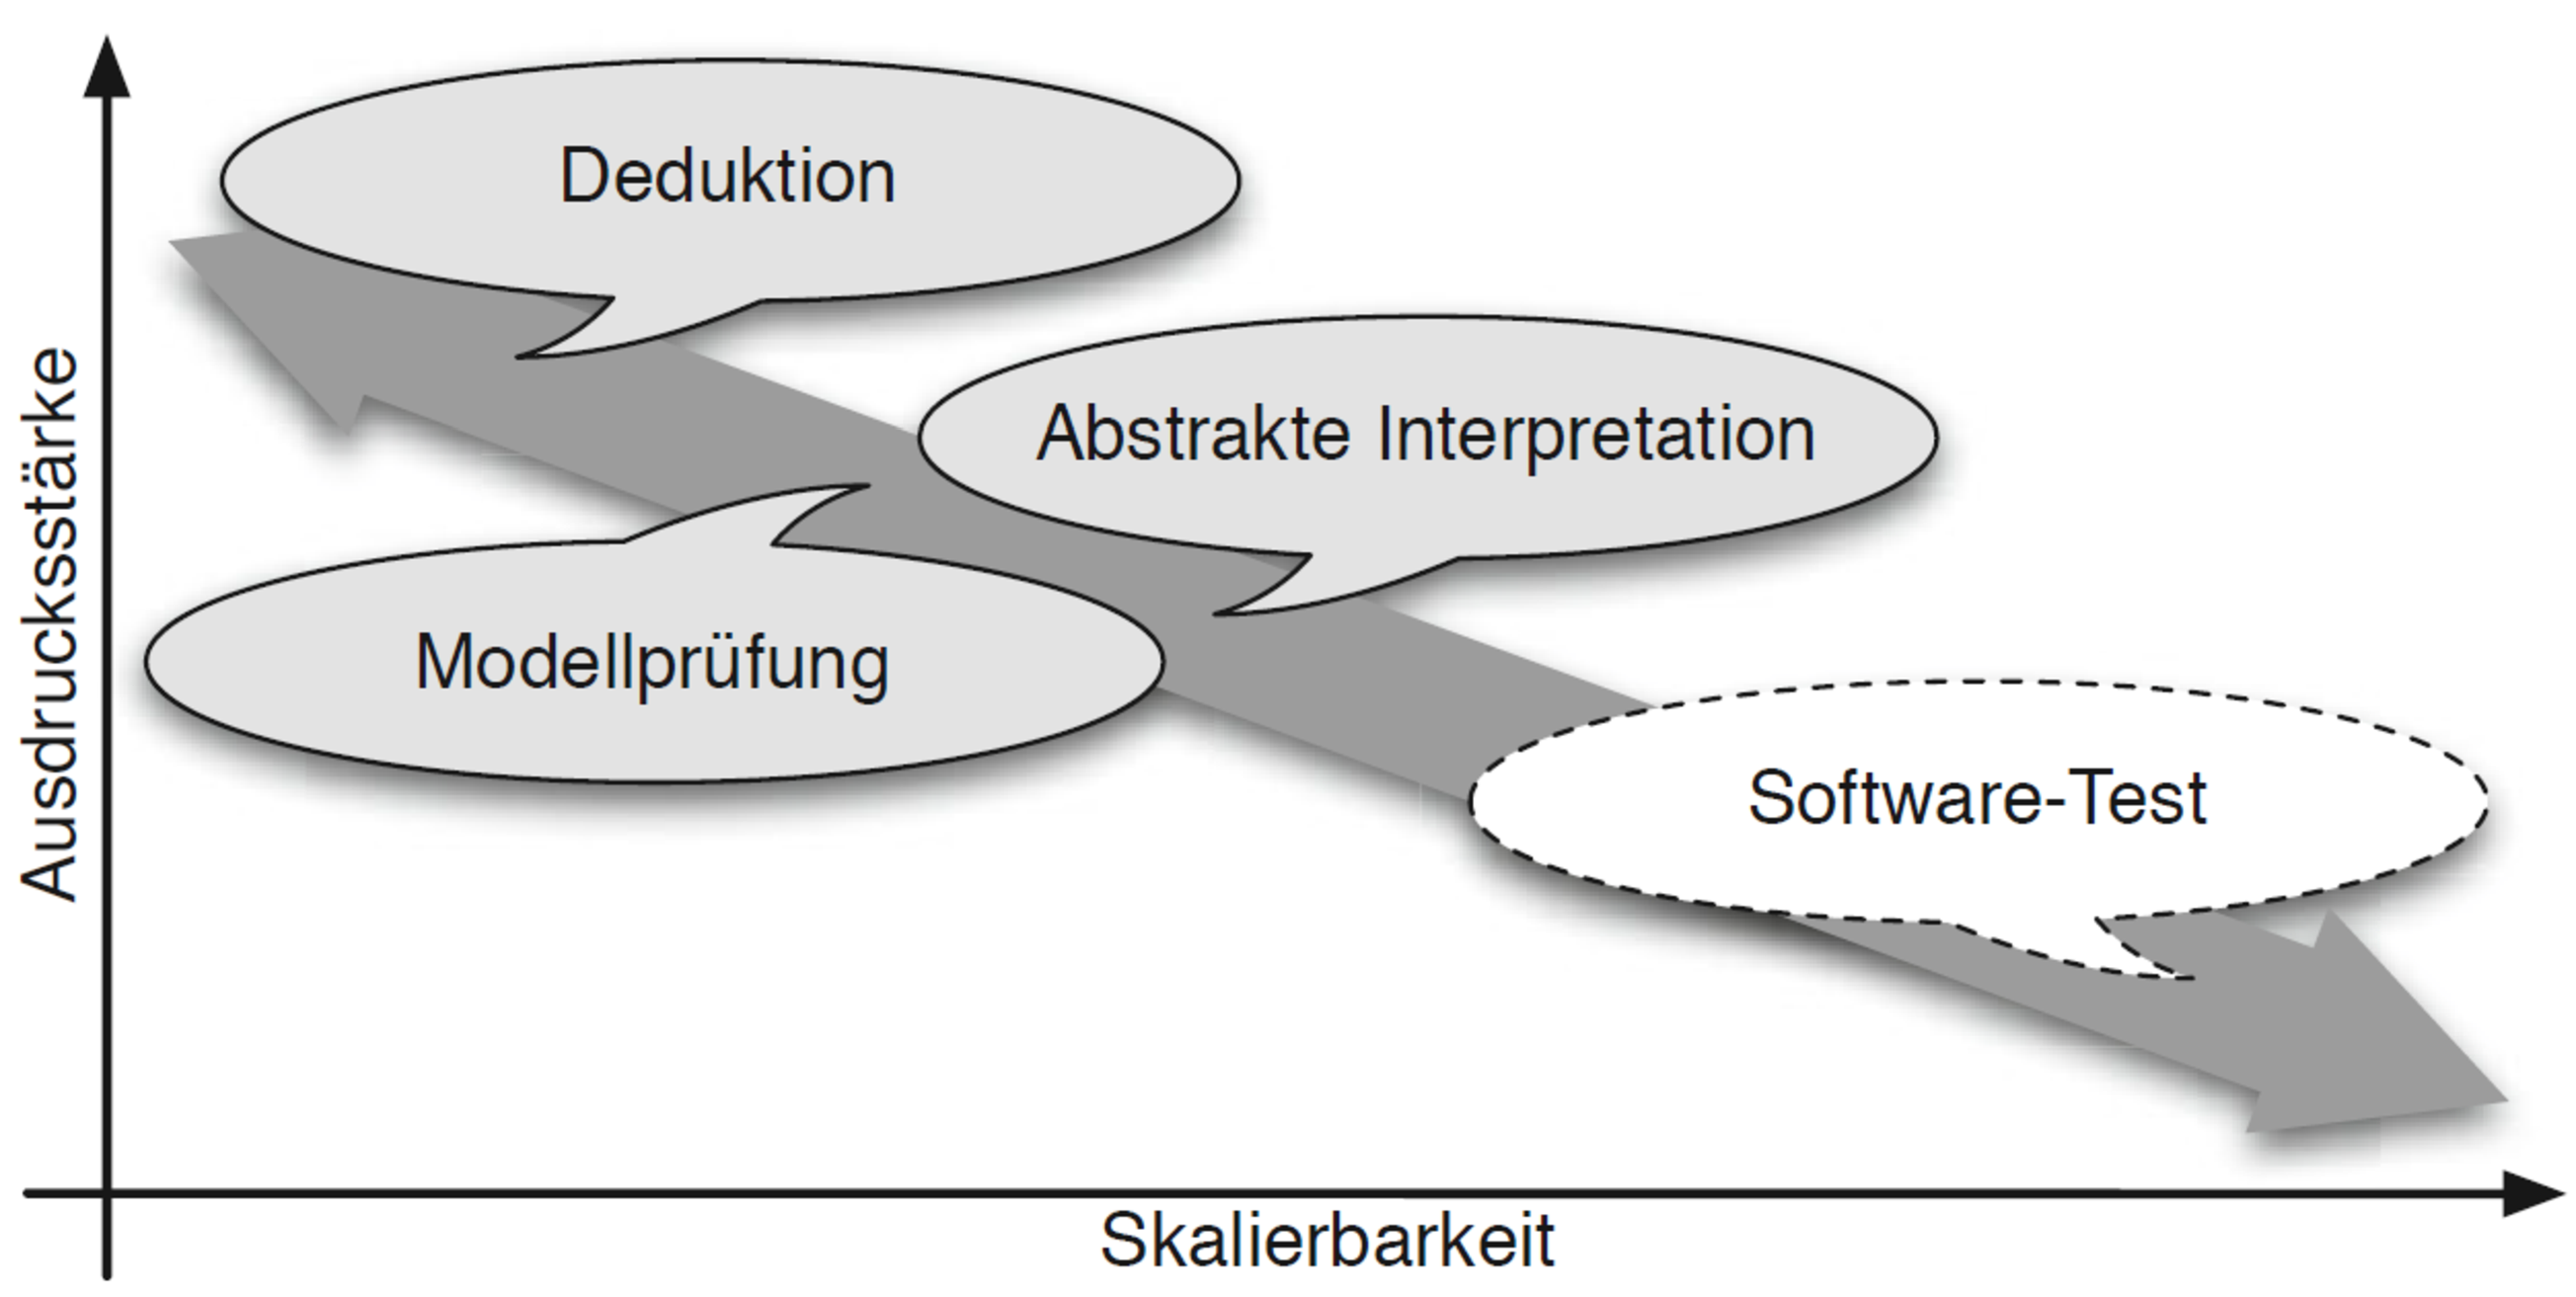
\includegraphics[
    width=\textwidth,
    height=\textheight,
    keepaspectratio
  ]{resources/software-quali-verification.pdf}
  \caption{Verhältnis von Ausdrucksstärker und Skalierbarkeit der Verifikationstechniken}
  \label{software-quali-verification}
\end{figure}

\section{Continuous-Integration}

Continuous-Integration wurde sehr treffend beschrieben \footcite{fowler2006}

\blockquote {Continuous-Integration is a software development practice where members of a team integrate their work 
frequently, usually each person integrates at least daily - leading to multiple integrations per day. Each integration is 
verified by an automated build (including test) to detect integration errors as quickly as possible.}

Continuous-Integration wurde erstmals von Kent Beck als Teil einer Reihe von Praktiken des Entwicklungsvorgehens ``Extreme Programming''\footcite{kent1999} beschrieben. Dabei sollte die Integration der einzelnen Entwickler-Codeständen gefördert werden. Entwickler sollen ihre Änderungen täglich oder häufiger abgleichen und durch einen automatisierten Vorgang als lauffähig beweisen. Damit konnten Fehler nahe des Zeitpunkt des Auftretens gefunden werden. Fehler die erst mit der Integration von Änderungen anderer Entwickler auftreten, können so gefunden werden. Damit fordert Continuous-Integration eine aussagekräftige Testabdeckung mit automatischen Tests. Des Weiteren können und sollten Entwickler einen entdeckten Fehler direkt beheben, da sonst alle anderen Teammitglieder behindert werden.

Die Arbeitsweise alle Änderungen auf einem Zweig zu sammeln und kontinuierlich zu integrieren, wird auch Trunk-Based-
Development genannt. Während Continuous-Integration und Trunk-Based-Development als getrennte Methodiken geführt werden
\footcite{trunkbaseddevelopment}, treten beide Begriffe häufig in Kombination oder synonym 
auf\footcite{fowler-feature-branch}.

Natürlich nutzt Continuous-Integration auch alle Vorteile, die im 
Kapitel~\ref{sec:automation-software}~\nameref{sec:automation-software} beschrieben werden. Modularisierung, 
Konfigurationsmanagement, automatische Erstellung und Wiederverwendbarkeit von Artefakten, sowie das Achten auf 
Testbarkeit der Anwendung. Die vollständige Erfüllung dieser Kriterien fordert und fördert eine gute Entwicklungskultur.

TODO: hatte humble das nicht sogar so gesagt? (quote?)
 
Dies ist einer der Gründe warum Continuous-Integration seit den Beschreibungen 
von Kent Beck so sehr an Akzeptanz und Bedeutung gewonnen hat.

Während die Vorteile von Continuous-Integration deutlich sind, gibt es auch Kosten die mit dieser Technik einhergehen. 
Die komplette Automatisierung erfordert einen erheblichen Aufwand in der initialen Einrichtung und einen häufig 
unterschätzten Aufwand in der Aufrechterhaltung. Gerade weniger wichtige Projekten oder Projekte unter besonders hohem 
Druck neigen dazu wichtige Bestandteile von Continuous-Integration zu vernachlässigen. Mögliche Symptome sind das sinken 
der Testabdeckung. Oder Teile des Konfigurationsmanagements werden umgangen und essentielle Abhängigkeiten von Hand 
gepflegt. Dieses Verhalten widerspricht offensichtlich der langfristigen Wertschöpfung und bricht mit den Prinzipien von 
Continuous-Integration. Menschliche Schwächen sind auch in Continuous-Integration noch ein Problem. Mit regelmäßigem 
Training, Erfahrung und Selbstdisziplin kann dem entgegen gewirkt werden. In Kapitel~\ref{sec:human-fail} wird das Thema 
Entwicklerdisziplin erneut aufgegriffen und auf die Gratwanderung von gesunder Entwicklungskultur und destruktiver 
``blaming culture'' eingegangen.

\section{Virtualisierung}

Im Kapitel ~\ref{sec:automation-software}~\nameref{sec:automation-software} wurden bereits Stärken von Virtualisierung 
genannt. Gerade bei der vollautomatisierten Bereitstellung von System können Stärken der Virtualisierung genutzt werden.

Virtualisierung bietet eine Abstraktionsschicht für verschiedene Komponenten. Dies ermöglicht Abhängigkeiten zu Hardware, 
Software und deren Konfiguration transparent zu gestalten. Der unter Programmierern bekannte Spruche ``It works on my 
machine'' verdeutlicht das Problem. Häufig benötigen Komponenten einer Softwareanwendung andere Anwendungen um lauffähig 
zu sein. Abhängigkeiten zum Betriebssystem, zu Software von Drittanbietern oder zu Hardwarekomponenten sind Bestandteil 
vieler Softwareanwendungen. Im Verlauf der Anwendungsentwicklung ist es daher wichtig diese Abhängigkeiten zu 
beschreiben. Zudem ist es immer wieder notwendig alle Abhängigkeiten in Form eines Systems zur Verfügung zu stellen.

Die manuelle Bereitstellung diese Systeme ist aufwändig und verzögert damit zusammenhängende Entwicklungsabläufe. Eine 
automatisierte Erstellung und Bereitstellung der benötigten Systeme ist daher empfehlenswert. Um unerwartetes Verhalten 
der auf den Systemen ausgeführten Anwendungen zu vermeiden, sollten die Systeme vollständig beschrieben sein. Die 
automatische Generierung der virtuellen Umgebung und die Ablage in gepackter Form in einem Archiv bietet weitere 
Vorteile. Der Zugriff auf die Virtualisierung und damit die Bereitstellung der Systeme wird dadurch besonders transparent 
und wenig aufwändig.

Durch die Virtualisierung kann ein System reproduzierbar und schnell in einem vorher definierten Zustand bereit gestellt werden. Dies verkürzt Arbeitsabläufe für den Test einer Anwendung. Zum einen können schnell Änderungen an der Anwendung getestet werden, zum anderen kann die Anwendung in zahlreichen Konfigurations- und Abhängigkeitskombinationen getestet werden.

\subsection{Virtualisierung mit Virtual-Machines}

Virtualisierung mit Virutal-Machines abstrahiert eine vollständige Systemumgebung. Diese ermöglicht unter anderem ein Betriebssystem innerhalb eines anderen Betriebssystems zu betreiben. Da eine vollständige Systemumgebung mit Hardwarekomponenten emuliert wird, lassen sich Anwendungen auf verschiedenen Virtual-Machines komplett unabhängig voneinander betreiben. 
Durch die Vollständigkeit der Virtualisierung ist der Systemressourcenverbrauch signifikant höher als beim Betrieb einer Anwendung in einem nicht virtualisierten System. Virtuelle Maschinen skalieren somit gut in Erstellung und Verwaltung. Im Gegensatz dazu skaliert der Systemressourcenverbrauch deutlich schlechter. Durch den geringeren Verwaltungsaufwand können dennoch große Cluster kosteneffizient betrieben werden, wie viele Cloud-Services zeigen\footcite{a-cloud-guru-cost}.

\subsection{Containerverwaltung mit Docker}

Docker ist keine Virtualisierung im eigentlichen Sinne. Ein Docker-Container ist eine standardisierte Umgebung in der ein Anwendung laufen kann. Ein Docker-Server verwaltet die Docker-Container und regelt deren Sicherheit- und Leistungsbedürfnisse. Docker läuft somit als Anwendung auf einem System und ist an dessen Spezifikationen für Betriebssysteme und Hardwarekomponenten gebunden\footcite[Why are containers important][]{learn-docker}.

Anwendungen werden in Form von Docker-Images abgespeichert und können dann in unbegrenzt vielen Docker-Container ausgeführt werden. Änderungen im Inhalt des Docker-Containers sind auf diesen beschränkt und haben keinen Einfluss auf das Docker-Image aus dem er erstellt wurde.

Mit Docker und virtuellen Maschinen wurden zwei Möglichkeiten geschaffen Software weiter zu vereinheitlichen. Standardisierung ist eine wesentliche Basis für Modularisierung und Automatisierung.

\section{Dezentrale Versionierung mit Git}

Im Kapitel~\ref{subsec:konfigurationsverwaltung} Konfigurationsverwaltung wurde bereits auf das Thema Versionsverwaltung 
eingegangen. Als das populärste System im Open-Source-Bereiche\footcite{openhub-pie-chart} und eines der großen Systeme 
im kommerziellen Bereich\footcite{g2crowd2018}, wird nun anhand von Git erläutert, wie die dezentrale Versionsverwaltung 
grundlegend verwendet wird. Außerdem kommen einige git-spezifische Merkmale hinzu, welche bei der visuellen Aufbereitung 
wichtig werden.

Git wurde vom Linux-Schöpfer Linus Torwalds im April 2005 initiiert, aus der Not heraus sich vom vorher verwendeten 
``BitKeeper''-System zu lösen, da diese nicht mehr mit der eigenen Open-Source-Lizenz in Einklang zubringen war. Git 
wurde von vornherein als verteiltes, vor Verfälschungen sicheres und effizientes Versionsverwaltungssystem entworfen. 
Diese Eigenschaften und die Software-Plattform ``GitHub'', machten Git in den letzten 13 Jahren zum de-facto Standard für 
Versionsverwaltung\footcite{heise-torvald-git2015}.

Als dezentrales Versionsverwaltungssystem ist einer der großen Vorteile von Git, dass die vollständige Historie der 
Dateien lokal verfügbar ist. Während zentrale Versionsverwaltungssysteme immer einen dedizierten Server benötigen, können 
dezentrale Varianten über Peer-To-Peer-Schnittstellen kommunizieren. Diese Eigenschaft sorgt neben einer hohen 
Ausfallsicherheit und Informationsredundanz, auch für eine hohe Flexibilität und die Möglichkeit zahlreiche Arbeitsweisen 
von Softwareentwicklern zu unterstützen.

\subsection{Definition und Verwendung der Git-Artefakte}

Die Verwendung von git gestaltet sich vergleichsweise einfach. In wenigen Schritten kann Git installiert \footcite{git-scm-install} und mit der Verwendung begonnen werden. 
Git nutzt bestimmte Artefakte um seine Aufgaben zu erfüllen. Darunter Repositories, Commits, Branches und Tags. Zudem 
werden Mechanismen bereitgestellt um mit diesen Artefakten zu interagieren. Neben zu erwartenden Mechanismen wie 
Hinzufügen und Löschen, werden auch Speichern- und Ladeaktionen (``push'' und ``pull) angeboten\footcite{git-essentials-2017}.

\begin{figure}[htbp]
  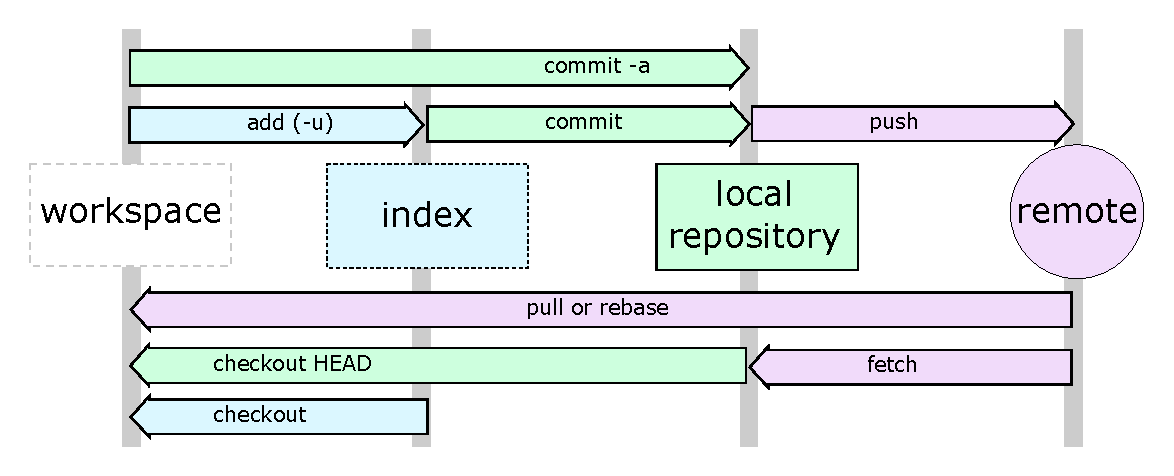
\includegraphics[
    width=\textwidth,
    height=\textheight,
    keepaspectratio
  ]{resources/git-workflow.pdf}
  \caption{Git-Workflow}
  \label{git-workflow}
\end{figure}
Die Grafik~\ref{git-workflow} stellt das Zusammenspiel der Artefakte und den Standard-Git-Worflow\footcite{osteele-git-workflow} dar.

\paragraph{Repositories} sind die größte Verwaltungseinheit in Git. Diese enthalten alle Git-Objekte, wie Referenzen, 
Commits, Trees, Blobs, sowie die lokale Konfiguration. Repositories können andere Repositories referenzieren oder 
referenziert werden, dabei können viele gängige Protokolle verwendet werden (http, ssh, ftp, absolute Pfade)

\paragraph{Commits} sind zeitlich determinierte, persönliche und kommentierte Referenzen auf einen konkreten Arbeitsstand 
(``Snapshot'') des Repositories. Ein Commit kann auf mehrere Eltern-Commits verweisen und kann von beliebig vielen 
anderen Commits referenziert werden. Bei Betrachtung aller Commits, bilden dieser daher einen gerichteten Graphen. 
Mehrere Eltern-Commits entstehen bei der Zusammenführung von Branches.

\paragraph{Branches} sind, im Gegensatz zu vielen anderen Versionverwaltungssystemen, in Git lediglich Verweise auf einen 
bestimmten Commit. Wenn ein Branch aktiv ist, dann wird mit jedem Commit auf diesem Branch, der Verweis auf den neuen 
Commit aktualisiert.

\paragraph{Tags} sind genauso wie Branches einfache Verweise auf einen Commit, allerdings verändert sich die Position 
eines Tags nach einem Commit nicht.

\paragraph{Remotes} sind Verweise in der Konfiguration eines Repositories auf andere Repositories. Dies wird im 
allgemeinen genutzt um Änderungen von dort zu holen oder dorthin zu bewegen. Es können beliebig viele Remotes für jedes 
Repository definiert werden. Zudem kann beliebig definiert werden, welche Branches von einem Repository Änderungen 
erhalten oder dieses aktualisieren.

\paragraph{Blobs} sind die komprimierten Inhalte einer Datei.

\paragraph{Trees} sind Referenzen von Blobs, und stellen damit im einfachsten Fall eine Ansicht eines Verzeichnisses und 
seiner Dateien dar.

\paragraph{Hashes} sind im allgemeinen Abbildung einer großen Abbildung von Zeichen auf eine deutlich geringere Menge. 
Die Abbildung führt immer zur gleichen Ergebnismenge. In Git werden Hashes als allgemeine Referenzierungsmöglichkeit 
verwendet. Alle Relationen werden darüber beschrieben und sind daher über alle Repositories gleich. Git verwendet für die 
Bildung der Hashes den SHA1-Alogrithmus. Die Forderung statt des SHA1- den SHA256-Algorithmus zu verwenden, wurde 
abgelehnt. Linus Torvalds schätzt die Sicherheitsbedenken als nicht zutreffend ein\footcite{git-sha-torvalds}. Diese 
Aussage wurde auch von GitHub bestätigt\footcite{git-sha-github}.

\subsection{Interne Arbeitsweise}

Git verwendet intern einen Mix aus Referenzen, Indexierung, Komprimierung und Hashing. Zudem werden keine 
Differenzmengen, wie etwa in Subversion abgelegt, sondern immer vollständige Dateiinhalte. Für manche Projekte, wie das 
Mozilla-Projekt\footcite{kernel-git-svn} kann dies einen Speicherplatzreduktion erreichen. Im Allgemeinen kann dies aber 
nicht bestätigt werden\footcite{svn-vs-git}. Durch die vollständige Speicherung der Inhalte in jedem vernetzten Git-
Repository, ist der Speicherbedarf insgesamt höher. Insbesondere für große Dateien, mit nur geringfügigen Änderungen 
ergeben sich deutliche Unterschiede zu Versionssystemen mit Differenzmengen. Für schlecht komprimierbare Dateien oder 
Dateien mit schlechten Differenzmengen, wie etwa Binärdateien, sollte allerdings grundsätzlich eher einer Artefakt-
Repository in Betracht gezogen werden.

Um die interne Arbeitsweise von Git zu erläutern, müssen die Zusammenhänge von Commits, Trees, Blobs und Hashes 
verdeutlicht werden.

Die Git-Objekte werden von Git immer anhand ihres Hashes abgelegt. Dabei wird ein 40-Stelliger SHA1-Hash verwendet. Die 
notwendigen Stellen zu Referenzierung sind aber häufig deutlich geringer, so können im allgemeinen Gebrauch deutlich 
verkürzte Zeichenketten verwendet werden. Im allgemeinen etwa 5 Stellen oder bei großen Projekten, wie dem Linux-Kernel, 
12 Stellen.

Der Hash von Blobs ist eine Abbildung ihres Inhaltes. Daher werden Dateien mit den gleichen Inhalt auch immer auf den 
gleichen Blob abgebildet, unabhängig vom Verzeichnis in dem sie sich befinden oder wie oft sie geändert wurden. Da ein 
Blog nur die Abbildung des Inhaltes der Datei ist, führen Merkmale wie Zeitstempel oder Dateirechte zu keiner Änderung 
des Hashes.

Wie auch beim Blob sind Trees nur eine Abbildung ihres Inhaltes. Da Trees aber als eine Art Verzeichnis zu verstehen 
sind, referenzieren Trees andere Trees und Blobs. Damit würde eine Folge von Commits, die zuerst eine Datei erzeugt und 
schließlich wieder entfernt, am Ende wieder auf den gleichen Tree verweisen.

Commits schließlich verweisen auf einen oder mehrere Vorgänger-Commits, einen Tree, einen Autor und einen Commiter. Im 

Dieser einfache, gut skalierbare Aufbau ermöglicht eine sehr leichtgewichtige Erstellung von Branches und damit 
zahlreiche flexible Arbeitsweisen.

\subsection{GitHub-Workflow}

GitHub ist heute die größte Plattformen für quelloffene Softwareprojekte\footcite{github-marketshare-datanyze}. Durch die 
rasante Verbreitung von Git, wurde GitHub bei Open-Source-Projekten schnell zur Alternative für Sourceforge
\footcite{heise-github-2011}. Damit einhergehend hatte der GitHub-Workflow\footcite{github-workflow-intro} auf die Git-
Gemeinschaft hohen Einfluss.

Der GitHub-Workflow ist eine einfache Arbeitsweise, die auf Branches und manuellen Begutachtungen(Reviews) basiert. 
Änderungen gelangen nur zurück auf den Hauptstrang, wenn sie zuvor einem Review unterzogen worden. Dieser Schritt ist ein 
entscheidender Unterschied zum Trunk-Based-Workflow der mit Continuous-Integration propagiert wird, da hier der Code-
Review erst nach der Integration mit dem Hauptzweig durchgeführt werden kann.

\subsection{Gitflow}
\label{subsec:gitflow}

Gitflow ist ein weiterer bekannter Workflow mit Git\footcite{nvie-git-branch-model}. Im Gegensatz zum simplen GitHub-
Workflow liegt beim Gitflow der Schwerpunkt auf der Erstellung eines Releases, also einer Menge an Commits, häufig auch
von verschiedenen Autoren.

In Anlehnung an viele bekannte Modelle unterscheidet Gitflow zwischen Produktivzweig(master), außerplanmäßiger 
Anpassung(hotfix), Auslieferungszweig(release), Entwicklungszweig(development) und zahlreichen Feature- und Bug-Zweigen.

Gitflow unterscheidet wie viele andere Git-Arbeitsmodelle zwischen langlebigen und kurzlebigen Branches. Die langlebigen 
Branches sind hierbei ``master'' und ``development''. Alle anderen Branches sind kurzlebige Branches(``supporting 
branches''), die immer erst erstellt werden, wenn sie notwendig sind und gelöscht werden, sobald sie ihren Zweck erfüllt 
haben.

\begin{figure}[htbp]
  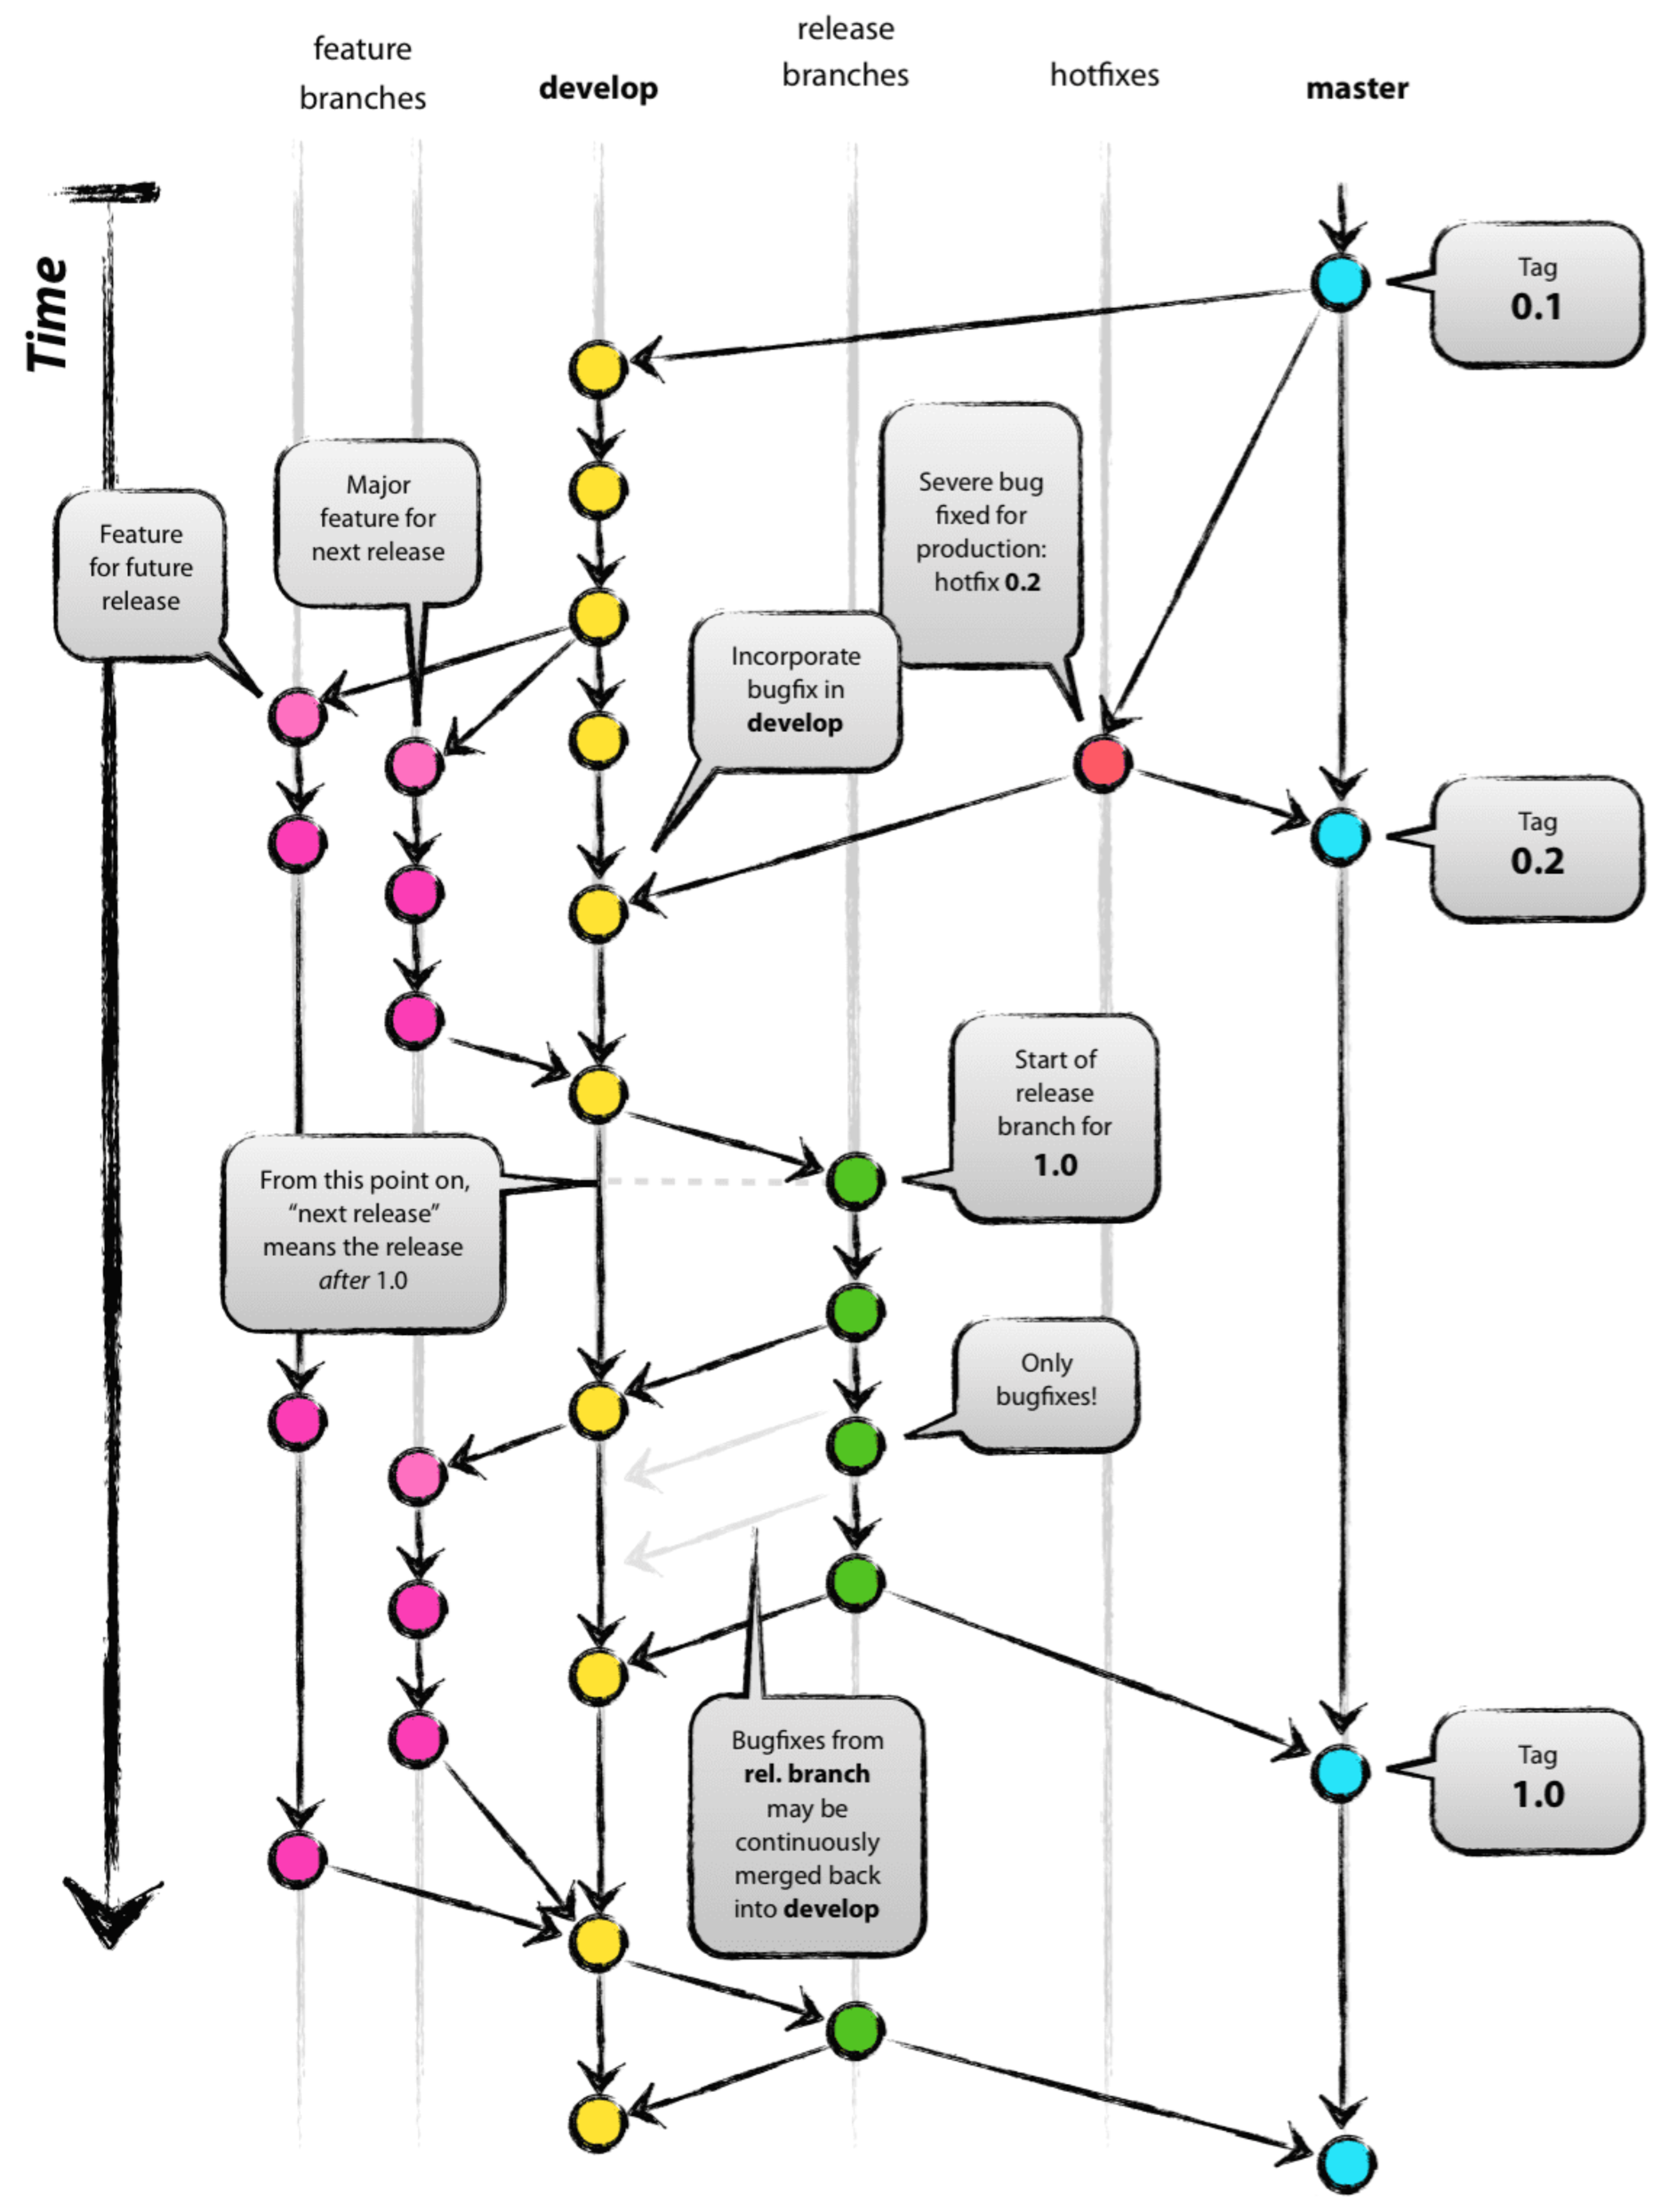
\includegraphics[
    width=\textwidth,
    height=\textheight,
    keepaspectratio
  ]{resources/git-flow.pdf}
  \caption{Gitflow-Workflow}
  \label{git-flow}
\end{figure}
Der konkrete Arbeitsfluss wird in der Abbildung~\ref{git-flow} zusammengefasst. Es wird deutlich dass nur Commits von 
Release- und Hotfix-Branches auf den Master-Branch gelangen können. Desweiteren ist herauszustellen, dass nach der 
Erstellung des Release-Branches keine Änderungen mehr vom Development-Branch zugeführt werden. Diese Trennung der 
Änderungsflüsse führt dazu, dass bereits an neuen Themen gearbeitet werden kann, ohne dass der Release behindert wird. 
Des Weiteren ist klar geregelt, dass alle Features immer erst im Development-Branch integriert werden müssen.

\section{Feature-Branches}
\label{sec:feature-branches}
Die Idee hinter einem Feature Branch ist, dass für jedes neue Merkmal, beziehungsweise für jede neue Anforderung ein 
neuer Branch in der Versionsverwaltung erstellt wird. Ziel von Feature-Branches ist die Isolierung von Änderungen, um die 
anderen Zweige nicht zu blockieren und Änderungen erst nach Test und Abnahme zusammen zu führen. Dabei sollen mehrere 
Änderungen parallel entwickelt werden können, ohne dabei zu einem bestimmten Zeitpunkt alle Änderungen in einen 
Hauptzweig übernehmen zu müssen.

Prinzipiell ist diese Technik unabhängig von der verwendeten Versionsverwaltung, erhielt aber vor allem durch dezentrale 
Versionsverwaltungssysteme an Bedeutung. Der Grund dafür liegt in der deutlich einfacheren und weniger aufwändigen 
Erstellung von Branches und deren Zusammenführung.

Feature Branching wird kontrovers diskutiert\footcite{fowler-feature-branch}\footcite{ci-is-dead}\footcite{fb-revisited}. 
Dabei wird angemahnt, dass die Abspaltung in einen Branch, das Problem der Zusammenführung von Codeänderungen nicht 
behebt, sondern verschlimmert. So wird der Aufwand, der benötigt wird um zwei Verzweigungen zusammen zuführen, potentiell 
immer höher, um so mehr Änderungen hinzukommen. Die Aufwandserhöhung kann soweit gehen, dass ein psychologischer Faktor 
hinzukommt, der die Entscheidung zur Zusammenführung weiter belastet. Diese Zusammenführung wird dann auch als ``big 
scary merge'' oder ``big bang merge'' bezeichnet.

Kontrovers dazu wird die hervorgehoben, dass Feature-Branches Blockaden im Arbeitsfluss vermeiden und die Angst vor dem 
``big scary merge'' durch Entwicklerdisziplin und Automatisierung gemildert. Die Entwicklerdisziplin verlangt Feature-
Branches nur für kleine Änderungen zu verwenden und durch Hilfe von Automatisierung schnelle Rückmeldung über die 
Codequalität zu erhalten. Des Weiteren werden durch moderne ``pull based''\footcite{github-about-pull}
Verzweigungsstratgien Entwickler dazu angehalten Codeprüfungen durch andere Entwickler einzufordern. Diese 
Lösungsstrategien werden in Kapitel~\ref{ch:visu_meth} weiterführend betrachtet.